%% main.tex
%% Copyright 2022 skyleaworlder
%
% This work may be distributed and/or modified under the
% conditions of the LaTeX Project Public License, either version 1.3
% of this license or (at your option) any later version.
% The latest version of this license is in
%   http://www.latex-project.org/lppl.txt
% and version 1.3 or later is part of all distributions of LaTeX
% version 2003/12/01 or later.
%
% This work has the LPPL maintenance status "maintained".
%
% This Current Maintainer of this work is skyleaworlder.
%
% This work consists of all the *.tex and *.sty files in
%   https://github.com/TJ-CSCCG/Tongji-Beamer
\documentclass{ctexbeamer}

\usepackage{amsthm}
\usepackage{biblatex}
\addbibresource{reference.bib}
\setbeamertemplate{bibliography item}[text]

\usetheme{tongji}

%Information to be included in the title page:
\title[Visionary Art]{Visionary Art}
\subtitle{人工智能绘画分享站:项目开发里程碑3汇报}
\author[Software Engineering: Group 11]{
    2051857 曾诗容 —— 项目主管 + 前端开发人员, \\
    2052636 陈骁 —— ECS云服务器技术顾问 + 全栈开发人员, \\
    2050250 李其桐 —— 技术支持 + 全栈开发人员, \\
    2054080 林奕如 —— 需求分析师 + 前端开发人员, \\
    2053865 刘昱彤 ——  产品经理 + 前端开发人员, \\
    1751118 吴达鹏 —— 运维 + 全栈开发人员, \\
    2053868 于采篱 —— 项目主管 + 前端开发人员
}
\institute[CS Dept., CEIE, Tongji Univ.]{
    Computer Science and Technology Department, College of Electronic and Information Engineering(CEIE), Tongji University. \\
    同济大学\ 电子与信息工程学院\ 计算机科学与技术系\
}
\date{\today}

\begin{document}

\begin{frame}
    \titlepage
\end{frame}

%% introductioin.tex
%% Copyright 2022 skyleaworlder
%
% This work may be distributed and/or modified under the
% conditions of the LaTeX Project Public License, either version 1.3
% of this license or (at your option) any later version.
% The latest version of this license is in
%   http://www.latex-project.org/lppl.txt
% and version 1.3 or later is part of all distributions of LaTeX
% version 2003/12/01 or later.
%
% This work has the LPPL maintenance status "maintained".
%
% This Current Maintainer of this work is skyleaworlder.
%
% This work consists of all the *.tex and *.sty files in
%   https://github.com/TJ-CSCCG/Tongji-Beamer
\section{引言}
    \begin{frame}
    % “无序列表” 与 “有序列表” 使用
    \frametitle{引言}
        \footnotesize
        \begin{block}{项目提出背景}
            \begin{itemize}
                \item 	当前,ChatGPT已经发布并且对公众开放了服务接口,这无疑标志着一个人工智能的新纪元已然到来。通过ChatGPT的强势赋能,使得许多传统工作流都得到了极大的颠覆与创新,在达到更高效率的同时也能够确保质量。本项目正是在这一背景下,基于ChatGPT的公开API接口,搭建一个能够根据用户的自然语言描述需求,自动生成Markdown格式文档,然后通过Markdown解析器处理文件文本内容从而生成ppt的软件系统,从而能够在人们的实际文档设计与编写工作中,以一个可靠软件助手的姿态提供辅助,有效提升人们的工作效率。
            \end{itemize}
        \end{block}

        \begin{block}{项目意义}
            \begin{enumerate}
                \item 为响应在互联网传统工作方式中,企业内部、学生和个人对PPT文档的自动化生成和在线编辑需求而进行设计和开发。
                \item 为用户节省编辑成本,提升编辑效率,拥有广泛的应用前景。
                \item 对于其它竞品的相关功能特性进行研究分析,并且在其基础上进行精炼、完善,同时围绕核心业务设计并且实现额外的使用子功能模块。
            \end{enumerate}
        \end{block}
    \end{frame}


%% introductioin.tex
%% Copyright 2022 skyleaworlder
%
% This work may be distributed and/or modified under the
% conditions of the LaTeX Project Public License, either version 1.3
% of this license or (at your option) any later version.
% The latest version of this license is in
%   http://www.latex-project.org/lppl.txt
% and version 1.3 or later is part of all distributions of LaTeX
% version 2003/12/01 or later.
%
% This work has the LPPL maintenance status "maintained".
%
% This Current Maintainer of this work is skyleaworlder.
%
% This work consists of all the *.tex and *.sty files in
%   https://github.com/TJ-CSCCG/Tongji-Beamer
\section{项目技术债}
    \begin{frame}
    % “无序列表” 与 “有序列表” 使用
    \frametitle{项目发布测试反馈与issue提取}
        \footnotesize
        \begin{block}{相关问题}
            本小组基于迭代2项目发布系统测试的反馈,结合答辩过程中与甲方沟通的相关情况,经过迭代3会议讨论,提取了以下问题:
            \begin{itemize}
                \item 在高并发情景下,绘图请求切换模型过多可能导致Stable Diffusion服务缓存池溢出,导致服务崩溃
                \item 模型查询、模型下载、模型上传等功能模块的后端接口由于数据库事务设计不当,存在性能瓶颈,导致用户体验不佳
                \item SD服务生成图片存在合法性问题,部分图片中出现了不合理的色块、扭曲的图像结构和我国法律法规禁止在互联网平台上传播的敏感内容
                \item 前端交互逻辑中存在不合理点,例如搜索界面的搜索按钮应该支持通过键盘按键触发,而不是需要用户手动点击;某些按钮功能提示缺失等
                \item 配置的ECS服务器由于硬件条件限制存在性能瓶颈,在高并发情景下的请求响应与处理可能由于硬件瓶颈失败
            \end{itemize}
        \end{block}
    \end{frame}

    \begin{frame}
    \frametitle{项目发布测试反馈与issue提取}
        \footnotesize
        \begin{block}{解决方案}
            本小组针对以上问题,在迭代3开发会议上进行讨论,最终提出了以下解决方案:
            \begin{itemize}
                \item 优化SD服务缓存池策略,基于LRU合理设计缓存换出机制,保证缓存命中率的情况下尽可能减少缓存池溢出的可能性
                \item 在服务端DAO操作和数据库事务之间,添加Redis中间件缓存访问机制,采用旁路缓存策略,将数据库访问压力转移到Redis上,从而在涉及到大表join查询或者高并发事务情景下减少数据库访问压力
                \item 由小组的相关前端开发人员,在单元测试和集成测试中,重新从用户角度出发对于人机交互逻辑进行省察,从而以用户友好为核心导向,进一步优化前端界面交互逻辑的相关功能需求实现
                \item 由小组的相关SD服务开发与维护人员,重新精读High-Resolution Image Synthesis with Latent Diffusion Models一文\cite{rombach2021highresolution},分别从prompt文本预处理方法、网络模型结构和权重文件检测的三个方向,对于<x>2image操作的生成图片合法性进行检测和优化
            \end{itemize}
        \end{block}
    \end{frame}






\section{本次里程碑任务}
\begin{frame}
    \frametitle{小组项目启动会工作项}
    \begin{itemize}
        \item 确定项目开发技术栈,搭建项目开发环境,使得相关框架能够正确集成并且运行。
        \item 根据甲方项目需求SRS文档,完成项目的需求分析,确定项目的主要功能,完成项目的功能设计与主要功能模块划分。
        \item 完成项目软件架构的逻辑设计和物理设计,主要包括数据库schema设计、索引设计、存储过程设计和视图设计,基于Restful API接口规范进行后端接口路由和功能设计等。
        \item 基于上述设计内容,使用华为云平台进行版本管理,将大功能模块设置为EPIC工作项,并且在Epic下抽取Feature,对于每个Feature进一步划分User Story,并且确定第一次迭代中需要实现的用户故事,最后分配工作到每位组员进行代码开发。
    \end{itemize}
\end{frame}

\begin{frame}
    \frametitle{工作项总览}
    我们小组在项目启动会中根据上述里程碑任务计划,详细讨论了项目的需求分析、软件架构设计、项目管理等内容,将设计细节落实到华为云工作项和开发文档,最终确定了本次里程碑任务的工作项,如下图所示:
        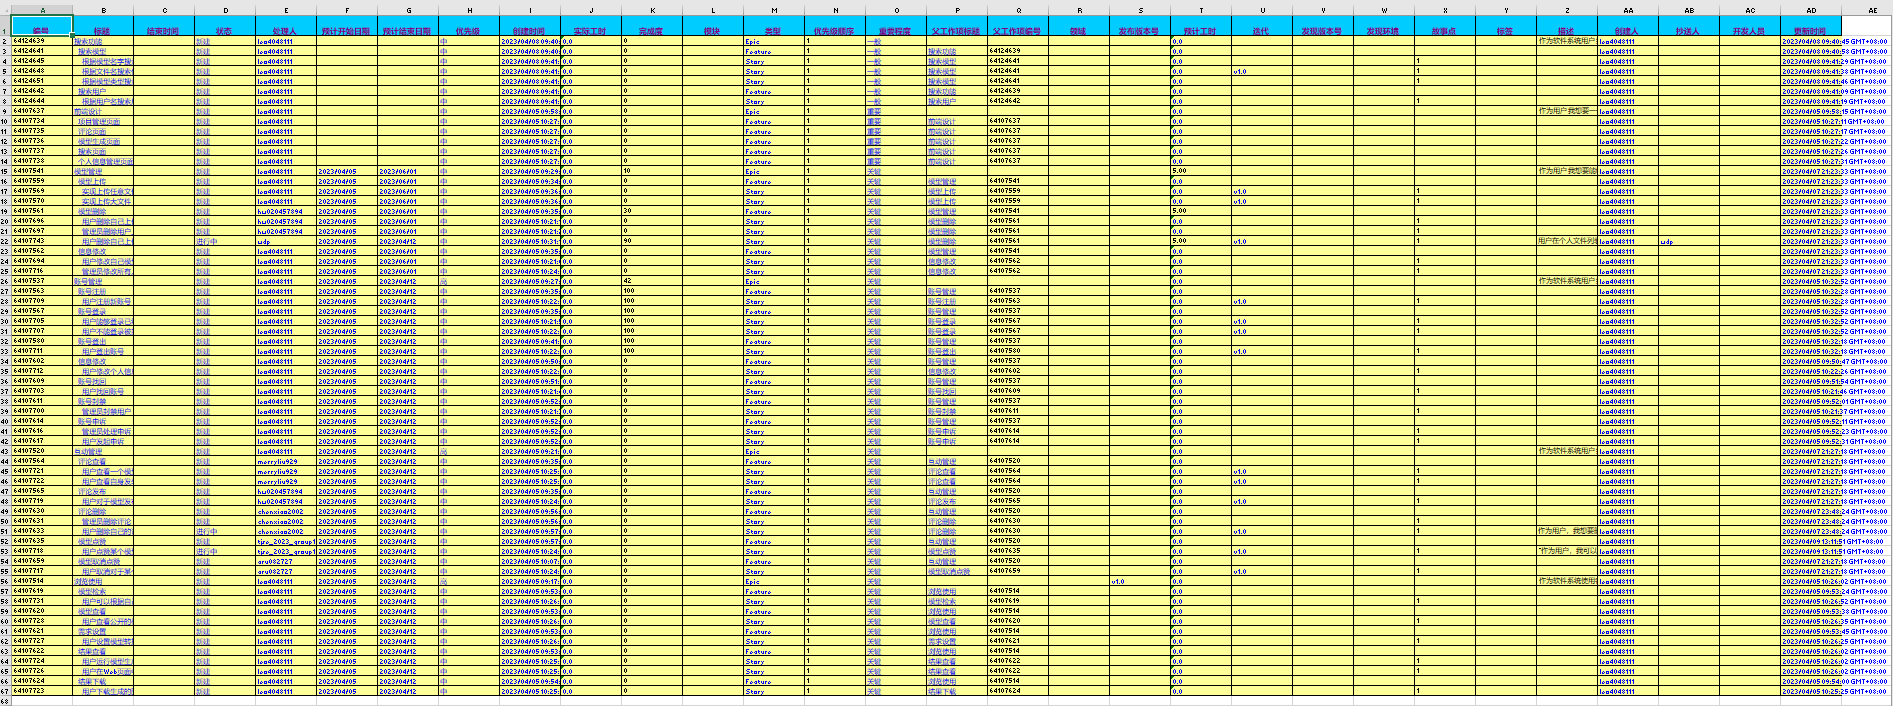
\includegraphics[width=2\textwidth]{contents/figure/work_items_overall.png}
\end{frame}

\begin{frame}
    \frametitle{项目技术栈}
    \begin{itemize}
        \item 主要开发语言:Python + HTML + CSS(SCSS) + JavaScript(Vue.js)
        \item HTTP服务器:Tornado
        \item 持久层框架:SQLAlchemy
        \item 数据库服务:MySQL + Redis
        \item 版本管理工具:Git
        \item 远程代码托管平台:华为云
        \item 接口管理与自动化测试工具:Apifox + Mock.js
    \end{itemize}
\end{frame}
\section{迭代三反思}
\begin{frame}
    \frametitle{目标和预期}
    \begin{itemize}
        \item 围绕甲方SRS需求文档为核心,高质量地完成相关功能需求的开发任务
        \item 围绕功能用例,时刻开展自动化测试,保证项目的稳定性和可用性
        \item 上线项目,邀请用户体验并给出测试反馈,收集用户意见和Bug反馈,为第三次迭代的内容规划提供参考
    \end{itemize}
\end{frame}

\begin{frame}
    \frametitle{信息和工具}
    \begin{itemize}
        \item 小组中对于相关功能需求分析实现,很大程度上参考了甲方提供的SRS需求文档,以及甲方提供的用例图,从而使得设计与实现内容与甲方需求最大程度地做到匹配
        \item 技术上,我们小组借助相关网络资料以及以往的开发经验,并且和相关从业专业人士进行沟通,充分对于当前行业的流行技术生态进行调研,选择最有利于敏捷开发的技术栈,从而使得项目开发效率得到了很大的提升
    \end{itemize}
\end{frame}

\begin{frame}
    \frametitle{困难与阻碍}
    \begin{itemize}
        \item 我们小组开发在迭代三遇到的最大的困难是在项目部署到服务器运行并测试时,遇到项目在实际的网络环境与本地环境下运行的差异,导致项目之前的许多功能实现可能在本地运行高效、良好,但是在网络环境下则由于网络带宽、高并发场景等原因,导致项目运行效率低下。这导致我们虽然很快地实现了相关的项目需求,但是依然需要负责相关功能模块的同学花费许多的时间对于原本功能实现的底层算法与代码逻辑进行优化,尽可能地降低算法对于系统资源的消耗。这也使得我们深刻意识到了实际生产环境下的项目开发与测试的重要性,以及对于项目的高效性、可用性的重视程度,让我们对于实际可用的工业化项目的敏捷开发流程有了更加深刻的认识。
    \end{itemize}
\end{frame}

\begin{frame}
    \frametitle{优势和创新}
    \begin{itemize}
        \item 得益于我们小组在迭代1中搭建的良好项目管理架构,我们在迭代三中进一步对于整个管理流程进行了完善,高度规范化了组员从功能开发、自动化测试、代码提交、审查、合并、部署、上线等整个项目开发流程,从而使得我们小组的开发人员能够更加专注于项目的功能实现,而不是处理各种由于项目流程管理不当产生的问题,使得我们小组的开发效率得到了进一步的提升。
        \item 我们小组在第一次迭代的基础上,继续完善技术栈,加入了Gradio + FastAPI的技术选型实现AI画图服务,使得我们小组的项目更加完善,功能更加丰富,同时也使得我们小组的项目更加具有创新性。
    \end{itemize}
\end{frame}

\begin{frame}
    \frametitle{结果和进度}
    \begin{itemize}
        \item 我们小组在每周的组会上,都会各自汇报本周自主开发以及集中开发中完成任务的情况,并且由会议记录人员进行统计。最终结果表明,小组在本次迭代中,完成了甲方提出的所有功能需求,并且在自动化测试方面也取得了很大的进展,使得我们小组的项目更加稳定可靠,结果还是比较让我们感到欣喜和自豪的。
        \item 我们小组的开发进度推进稳健,在下一次迭代(第三次迭代)中,主要将会根据当前的相关Bug反馈和用户需求,对于系统的一些相关问题进行修复和优化。
    \end{itemize}
\end{frame}

\begin{frame}
    \frametitle{情绪状态}
    \begin{itemize}
        \item 我们小组成员在迭代开发中,由于本身都还有其它大量的学业和工作压力,因此在迭代开发过程中,有时候会出现一些情绪波动,影响打出代码的可靠性和质量,导致提交时审查门禁不通过,被发回修改。但是我们小组成员都能够很好地调整自己的情绪,保持积极向上的心态,最终完成了本次迭代的开发任务。
    \end{itemize}
\end{frame}

\begin{frame}
    \frametitle{心得体会与开发意义}
    \begin{itemize}
        \item 通过本次迭代任务,我们小组成员之间的配合更加融洽并且具有默契,能够作为一个团队更加高效与良好地完成相关的项目开发任务,并且更加熟悉了类似的大型项目的开发流程与管理模式,为之后的下一次迭代乃至今后学习工作中的类似项目开发情景打下了良好的基础。
    \end{itemize}
\end{frame}
%%% summary.tex
%% Copyright 2022 skyleaworlder
%
% This work may be distributed and/or modified under the
% conditions of the LaTeX Project Public License, either version 1.3
% of this license or (at your option) any later version.
% The latest version of this license is in
%   http://www.latex-project.org/lppl.txt
% and version 1.3 or later is part of all distributions of LaTeX
% version 2003/12/01 or later.
%
% This work has the LPPL maintenance status "maintained".
%
% This Current Maintainer of this work is skyleaworlder.
%
% This work consists of all the *.tex and *.sty files in
%   https://github.com/TJ-CSCCG/Tongji-Beamer
\section{总结}
    \begin{frame}{总结}
        “永夜星弓” 系统已在我校试运行 2 个月。试运行期间,上报内卷行为 300'000 起,成功制止 280'000 次轻微内卷行为、10'000 次中等内卷行为以及 10'000 次重度内卷行为。

        \begin{center}
            感谢在毕业设计实现过程中提供指导的老师们!

            感谢在这百余天中一直陪伴我的家人和同学们!

            感谢这个美丽的世界给了我从大学毕业的机会!
        \end{center}

        \begin{center}
            谢谢各位!请多多指教!
        \end{center}
    \end{frame}

\begin{frame}{参考文献}
    \printbibliography
\end{frame}

\end{document}
